%% LyX 2.2.3 created this file.  For more info, see http://www.lyx.org/.
%% Do not edit unless you really know what you are doing.
\documentclass[english]{article}
\usepackage[T1]{fontenc}
\usepackage[latin9]{inputenc}
\usepackage{babel}
\usepackage{float}
\usepackage{amsbsy}
\usepackage{amstext}
\usepackage{graphicx}
\usepackage[unicode=true]
 {hyperref}

\makeatletter
\@ifundefined{showcaptionsetup}{}{%
 \PassOptionsToPackage{caption=false}{subfig}}
\usepackage{subfig}
\makeatother

\begin{document}

\title{SLAPS\\
\textbf{\large{}S}{\large{}parse }\textbf{\large{}L}{\large{}inear
}\textbf{\large{}A}{\large{}lgebra on a }\textbf{\large{}P}{\large{}artitioned
Global Address }\textbf{\large{}S}{\large{}pace}}

\author{Greg Meyer}

\date{Spring 2018}

\maketitle
Statement of original work:

All code in the source tree is original work by me for this project,
with the following exception: \texttt{catch.hpp} is the header-only
unit test framework Catch2, which can be found \href{https://github.com/catchorg/Catch2}{here}.

The source code is free and open source online at:

\href{https://github.com/GregDMeyer/slaps}{https://github.com/GregDMeyer/slaps}.

\section{Introduction}

SLAPS is a preliminary implementation of distributed sparse matrix-dense
vector linear algebra, making use of the PGAS library UPC++. It is
a header-only C++ library which currently defines two base class templates:
\texttt{Vec}, which implements a distributed dense vector, and \texttt{Mat},
which implements a distributed sparse matrix. These classes are described
below. All classes in SLAPS are templated, such that arbitrary data
types can be used for both the indices and the data. 

The most important features of SLAPS are:
\begin{itemize}
\item \textbf{Implicit} remote memory reads and writes in \texttt{Vec} class
\item \textbf{Efficient} SpMV through one-sided UPC++ communication, in
some cases outperforming PETSc's MPI implementation
\item \textbf{Header-only} library allows for ease of use and templated
API
\end{itemize}

\subsection{Background}

Linear algebra is a classic application for high-performance computing.
Often, the matrices involved in real-world problems are ``sparse''\textemdash many
of the elements are zero. Computations involving such matrices occur
in diverse fields, including physics and chemistry simulations, engineering,
and machine learning. My own research in the physics department studying
quantum many-body dynamics makes extensive use of large sparse matrices,
to solve high-dimensional linear algebra problems like eigensolving
and computing matrix exponentials. In my field and others, the matrices
and vectors are often so large that they must be distributed across
many processors.

One of the most important operations in sparse linear algebra is the
product of a sparse matrix and a dense vector (SpMV). This one operation
is the basis of a large class of algorithms, which can make use of
it to compute eigenvalues and functions of matrices. This work, SLAPS,
is a framework for efficient sparse matrix-dense vector multiplication.

The traditional approach to distributed memory SpMV is to distribute
the matrix and vector across processors' local memories, and then
use the message passing interface standard (MPI) for communication.
In general this can be quite efficient, but there are some downsides:
in particular, two-sided MPI requires both the sending and receiving
ranks to be prepared for that operation. When data access is unpredictable
(as it often is in sparse linear algebra), knowing when to check for
incoming MPI messages can be a difficult problem.

An alternative approach, the one pursued here, is to use a partitioned
global address space (PGAS). PGAS languages and libraries allow direct
reading and writing from a shared global memory, at the level of nodes'
network cards. This means that any process can read from the memory
locally stored on any node, without waiting for that node to check
for incoming requests.

\section{Implementation}

\textbf{Note:} the API is well documented in the class template declarations
at the beginning of each of the header files in the source tree. In
this document I describe just a subset of the member functions in
each class.

\subsection{\texttt{Vec}: a distributed dense vector}

The most obvious way to partition a dense vector across processors
without duplication is to split the indices as evenly as possible,
and give each rank a contiguous range. This is not the only way to
partition a vector, but it is the approach that will be taken here.\footnote{Perhaps a future version of SLAPS will include other vector partitionings.} 

\subsubsection{Data distribution}

UPC++ implements a partitioned global address space through global
pointers which affinity to one rank: the data is accessible from any
rank through remote put and get operations, but it resides locally
in one place. SLAPS thus stores the distributed vector as follows:
\begin{enumerate}
\item Each rank computes the distribution of vector indices (using the \texttt{partition\_array}
function in \texttt{utils.hpp}).
\item Each rank then allocates its own chunk of shared global memory, with
a size corresponding to the rank's range of indices returned from
the partitioning in step 1.
\item All ranks broadcast to all other ranks the global pointers to the
shared memory allocated in step 2, which are each saved locally in
an array.
\end{enumerate}
Now, since every rank has the global pointers corresponding to every
part of the vector, any rank can access any part of the distributed
vector through UPC++ remote get and put calls.

The partitioning of the vector is available to the user through several
functions. One can simply call \texttt{partition\_array} directly
to get the global partitioning, or one can use \texttt{Vec::get\_local\_range(I
\&start, I \&end)} and related functions to get the current rank's
local ownership. This is useful so that one can build a vector with
minimal remote writes, reducing unnecessary communication.

\subsubsection{Implicit remote memory access}

The main way of implicitly accessing remote memory elements is through
the \texttt{Vec::operator{[}{]}}. This method returns an object of
type \texttt{RData}, which is defined in \texttt{proxy.hpp}. The \texttt{RData}
object simply stores the global pointer to the value that has been
requested. Like everything in SLAPS, \texttt{RData} is templated with
index and data types \texttt{I} and \texttt{D}. The most important
functions defined are:
\begin{itemize}
\item \texttt{RData::operator= (const D \&val)}
\begin{itemize}
\item Set the data represented by this \texttt{RData} object. The future
for the write operation is chained to a global write future which
is a member of the governing \texttt{Vec} class (see \texttt{Vec::set\_wait()}
below). These operations are not atomic, and care must be taken by
the user to coordinates writes from different ranks.
\end{itemize}
\item \texttt{RData::prefetch()}
\begin{itemize}
\item Request the value from UPC++, and store the future internally.
\end{itemize}
\item \texttt{RData::get()}
\begin{itemize}
\item Wait on the future stored from \texttt{prefetch()} and return the
value when it's ready. If it has not been called, \texttt{prefetch()}
is called automatically.
\end{itemize}
\end{itemize}
The following additional operations are defined in the \texttt{Vec}
class:
\begin{itemize}
\item \texttt{Vec::set\_wait()}
\begin{itemize}
\item Wait for all writes performed through \texttt{operator=} to complete.
This is achieved by keeping an internal future in the \texttt{Vec}
class, and conjoining all futures from calls to \texttt{RData::operator=}
to it using \texttt{upcxx::when\_all}.
\end{itemize}
\item \texttt{Vec::read\_range(I start, I end, D{*} buf)}
\item \texttt{Vec::read\_range\_begin(I start, I end, D{*} buf)}
\item \texttt{Vec::read\_range\_end()}
\begin{itemize}
\item Request a range of contiguous values, even if they do not all reside
on the same rank. The second and third functions represent the asynchronous
version, in which work can be done between the calls to \texttt{begin}
and \texttt{end}.
\end{itemize}
\end{itemize}
Here is an example of remotely getting and setting data in SLAPS:
\begin{verbatim}
Vec<int, double> v(100);

/* get and set arbitrary values */
v[52] = 3.14;              // set on any process 
v.set_wait();              // wait for remote writes to complete

double val = v[52].get();  // get from any process

/* copy range into buf, even if it spans >1 processor */
v.read_range(0, 25, buf);  // copy v[0:25] into buf

/* all of the above can be done asynchronously */
auto remote_val = v[21];
remote_val.prefetch(); 
/* do other work */ 
double val2 = remote_val.get();
\end{verbatim}

\subsubsection{Vector functions}

Finally, two mathematical vector functions are implemented: 
\begin{itemize}
\item \texttt{Vec::norm()}, a vector 2-norm and 
\item \texttt{Vec::dot(const Vec\& b)}, the vector-vector dot product
\end{itemize}

\subsection{\texttt{Mat}: a distributed sparse matrix}

The other data structure implemented by SLAPS is the distributed sparse
matrix. The matrix elements are not stored in globally shared memory,
since for the SpMV implementations below, matrix elements do not need
to be communicated. Instead the matrix is partitioned across processors,
with each processor storing its portion in local memory.

\subsubsection{SpMV: Mechanics}

There are several possibilities for parallel sparse matrix data storage
formats and SpMV implementations. The vector partioning described
above suggests two implementations for partitioning and SpMV: a row-based
approach and a column-based approach (see Figure \ref{fig:rowcol}).

\begin{figure}
\subfloat[``Row-based'' method. Reads from all processes; writes to self.]{\begin{centering}
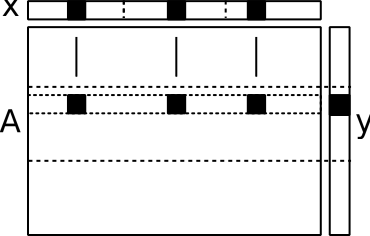
\includegraphics[width=0.4\textwidth]{row_based}
\par\end{centering}

}\hfill{}\subfloat[``Column-based'' method. Reads only from self; writes to all processes.]{\begin{centering}
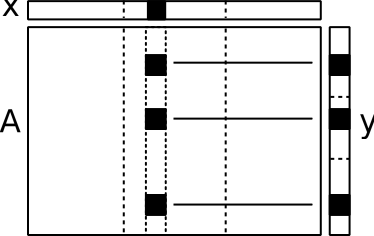
\includegraphics[width=0.4\textwidth]{column_based}
\par\end{centering}
}

\caption{\label{fig:rowcol}Sparse matrix partitioning schemes for SpMV. These
figures graphically represent the operations $\boldsymbol{y}=A\boldsymbol{x}$
(the product of matrix $A$ and vector $\boldsymbol{x}$ is being
written into vector $\boldsymbol{y}$). Dotted lines represent partitioning
across ranks ($p=3$ in this example).}
\end{figure}

For an MPI-based implementation of SpMV, the row-based formulation
has some subtleties. Communication must be done in two steps that
require coordination: first, send the indices to the process that
owns them, and second, receive the data. Both steps require the participation
of both ranks. The column-based method would seem superior, since
one can read from one's local array, then send computed values to
another rank in one step. The disadvantage of MPI in general, however,
is that the other rank must do extra work and coordination. It needs
to know when to receive the values and how many, and then needs to
sum the received values onto its array.

In our one-sided PGAS implementation the situation is quite different.
We can do the remote reads required for the row-based method efficiently,
and then we only need to write to our local array, which is extremely
efficient. In fact, the column-based method is \emph{worse} in a PGAS
implementation, because several processes might attempt to write to
the same remote value at once\textemdash requiring atomic operations.
UPC++ doesn't even define atomic operations for floating point data
types yet. It could be implemented using Remote Procedure Calls (RPC's),
but that defeats the benefit of having one-sided communication.

So, it is clear that a row-based approach (read from all, write to
self) is optimal for our PGAS implementation. With the partitioning
set we still have some freedom to implement the actual SpMV operation
in various ways, and currently four different methods are implemented
in SLAPS. These are accessible as derived classes of the base \texttt{Mat}
class, and are described below.

\subsubsection{\texttt{Mat}: the base matrix class}

The base class \texttt{Mat} defines operations and member data useful
for all matrix types. It determines the partitioning of rows, and
defines the user-visible functionality for setting nonzero matrix
elements. 

\textbf{Row partitioning}

The partitioning of rows is done in the same way as for the \texttt{Vec}
class: using \texttt{partition\_array} from \texttt{utils.hpp}.

\bigskip{}

\textbf{Setting matrix elements}

The setting of matrix elements occurs in two steps, only the first
of which is performed by the base \texttt{Mat} class: 
\begin{enumerate}
\item When users call \texttt{Mat::set\_element(I row, I col, D val)}, the
triple \texttt{(row, col, val)} is appended to a list of elements
stored by the \texttt{Mat} class. This storage corresponds to what
is referred to as COO (coordinate) format in the literature: just
a 1-D array of coordinates and values. This is good because it allows
quick matrix building, with no requirements that the users set elements
in any sorted order.
\item Derived classes define a \texttt{DerivedMat::setup()} function, which
takes the list of elements in COO format and translates it into the
storage format defined by the derived class (see below).
\end{enumerate}
\textbf{Methods defined by derived classes}

Derived classes are expected to define the \texttt{setup()} function
just described, and also the SpMV implementations:
\begin{itemize}
\item \texttt{DerivedMat::dot(Vec\& x, Vec\& y)}, which performs the operation
$\boldsymbol{y}=A\boldsymbol{x}$
\item \texttt{DerivedMat::plusdot(Vec\& x, Vec\& y)}, which performs the
operation $\boldsymbol{y}=\boldsymbol{y}+A\boldsymbol{x}$. 
\end{itemize}

\subsubsection{\texttt{CSRMat}: a base class for matrices using CSR storage format}

Derives from: \texttt{Mat}

\bigskip{}

CSR (compressed sparse row) format is one of the most ubiquitous sparse
matrix storage formats. It stores a jagged 2D array, for which the
first dimension is equal to the number of local rows. The second (jagged)
dimension contains each of the nonzero matrix elements in the corresponding
row, stored as a \texttt{(col, val)} pair. Here \texttt{col} is the
index of the column where the matrix element \texttt{val} sits.

The \texttt{CSRMat} class defines the function \texttt{CSRMat::setup()}
described earlier, which translates the raw COO format matrix elements
from calls to \texttt{Mat::set\_element} into CSR format. It stores
elements corresponding to local and remote reads from $\boldsymbol{x}$
separately for efficiency.

\subsubsection{\texttt{NaiveCSRMat}: SpMV the naive way}

Derives from: \texttt{CSRMat}

\bigskip{}

This class defines the \texttt{dot} operations in the naive way: just
iterate through the rows in the CSR format, requesting remote values
when we need them using the implicit remote gets defined in the \texttt{Vec}
class. This implementation is not expected to be very efficient because
it does not hide the latency inherent in the remote gets.

\subsubsection{\texttt{SingleCSRMat}: Naive SpMV, but with prefetching}

Derives from: \texttt{CSRMat}

\bigskip{}

This class defines effectively the same implementation as \texttt{NaiveCSRMat},
except that it explicitly prefetches values of \texttt{x} that will
be needed soon. It only uses x-values once before throwing them away,
possibly requiring the same value to be fetched many times. Thus it
may be inefficient in general, but efficient on very sparse matrices
in which only a few values are needed from \texttt{x} and they are
not reused. 

\subsubsection{\texttt{BlockCSRMat}: Remote values prefetched in blocks}

Derives from: \texttt{CSRMat}

\bigskip{}

This class prefetches entire portions of the \texttt{x} array, using
the asynchronous version of the \texttt{Vec::read\_range()} method,
and multiplies these values agains all relevant matrix elements at
once. These values are read regardless whether they need to be used
(i.e. the read is not packed, since that would require extra communication).
So, for denser matrices, this class is expect to outperform the \texttt{SingleCSRMat},
since it makes good reuse of values in the \texttt{x} array. However,
for very sparse matrices, a lot of extra values are communicated,
so at some level of sparsity we expect \texttt{SingleCSRMat} to be
faster.

\subsubsection{\texttt{RCMat}: a custom storage format for PGAS SpMV}

Derives from: \texttt{Mat}

\medskip{}

This is a custom format I implemented for this library, which I haven't
seen in any literature (though perhaps it has been implemented before
and I just haven't heard of it). I named it RC format for ``row-partitioned
columns.''\footnote{If anyone knows a name and previous implementation of this format,
I would love to hear it!} It combines the benefits of both the communication efficiency of
``\texttt{Single}'' and value reuse of ``\texttt{Block}'' implementations
above.

\begin{figure}
\begin{centering}
\includegraphics[width=0.9\textwidth]{RCMat}
\par\end{centering}
\caption{\label{fig:RCMat}The \texttt{RCMat} data structure.}
\end{figure}

The data structure is visually represented in Figure \ref{fig:RCMat}.
It is contained as a single array (implemented using a \texttt{std::vector})
of index-pointer pairs. The indices correspond to column numbers,
and the pointers point to an array of row index-value pairs. The data
structure is ``row-partitioned'' because the matrix elements contained
in it still only correspond to those that would be stored by the process
in a normal block-row format. 

This data structure has numerous advantages:
\begin{itemize}
\item For each (column index, pointer) pair, a single value from the \texttt{x}
array is multiplied by all the values in the (row index, value) array.
This makes provably optimal reuse of \texttt{x} values: each value
is fetched at most once, or zero times if it's not needed.
\item Since column indices are stored, no unnecessary \texttt{x} values
will be communicated.
\item For prefetching, the up-front storage of column indices makes it trivial
to calculate which indices will be needed soon, reducing computational
overhead.
\item Because matrix elements are still row-partitioned, all writes are
done locally.
\end{itemize}
I expect this data structure to perform well for both very sparse
and less sparse matrices: it makes optimal reuse of remote values,
but also does not do any unnecessary communication.

\section{Performance Results}

These performance results were obtained using NERSC's Cori supercomputer.
The measurements were performed using 1 process per node, for up to
32 nodes. The processor clock speed for the Haswell processors was
limited to 2.3 GHz, to reduce variance from turbo boost. For each
plot, all data points were obtained with the same set of nodes on
Cori, to keep the effects of topology constant. In addition to testing
the performance of SLAPS, the performance of the PETSc library's default
SpMV was measured for comparison.

For these preliminary tests, matrices with uniform nonzero density
across the row were used. For future testing, it would be interesting
to examine performance on matrices which are clustered near the diagonal,
or in bands.

For reproducibility, the build parameters for PETSc and SLAPS can
be found in the source tree, under the ``\texttt{benchmark/plots}''
directory. The benchmark code itself is in ``\texttt{benchmark/petsc}''
and ``\texttt{benchmark/slaps}''.

The plots are located in the appendix.

\subsection{Density scaling}

The density scaling plot can be seen in Figure \ref{fig:density}.
It explores the behavior of the various implementations as the density
of nonzeros in the sparse matrix is varied. This is not inherently
a ``parallel'' benchmark, since each point was computed with the
same number of nodes, but is important for understanding the scaling
behavior.

The x-axis of the plot is nonzero density per row (i.e. number of
nonzeros, divided by length of row). The y-axis is a measured of scaled
computational time. Since a less dense matrix would trivially run
faster, the runtime was divided by the density at each point to get
a measure of ``run time per unit density,'' which should be proportional
to FLOP/s.\footnote{In practice, the benchmark was just iterated a number of times equal
to the inverse density, to obtain equal computational work.}

These data points were all collected using 32 nodes, 1 processor per
node on Cori Haswell. The matrix dimension was held constant at 10,000.

\subsection{Strong scaling}

The strong scaling plot can be seen in Figure \ref{fig:strong}.

The x-axis is number of processors. Each processor was on a separate
node. The y-axis is the ``parallel efficiency,'' scaled to the performance
of the PETSc benchmark on one processor. It is

\[
\text{parallel efficiency}=\frac{\left(\text{PETSc }p=1\text{ runtime}\right)}{\left(\text{runtime}\right)\times\left(\text{\# processors}\right)}
\]

So, it's proportional to FLOP/s per processor.

For this computation, the matrix dimension was 30,000. It had a density
of $10^{-2}$ (one nonzero per 100 matrix elements), and the computation
was iterated 100 times for sampling.

\subsection{Weak scaling}

The weak scaling plot can be seen in Figure \ref{fig:weak}. 

The x-axis is the number of processors, and the y-axis is wall time
in seconds (not scaled in any way). The matrix dimension was set as
$d=30,000\times\sqrt{p}$, where $p$ is the number of processors
(giving a linear scaling of work with number of processors). The density
was $10^{-2}$, and the computation was iterated 50 times for sampling.

\section{Discussion}

First, for density scaling in Figure \ref{fig:density}, I had predicted
that the \texttt{BlockCSR} implementation would perform well for denser
matrices, but that the \texttt{RC} format would overtake it at low
matrix density, because it avoid unnecessary communication of unused
x-values. However, it appears that the extra efficiency gained from
communicating x-values in blocks completely dominates the costs of
communicating unnecessary ones.

In the strong scaling plot, Figure \ref{fig:strong}, both the \texttt{RC}
and especially the \texttt{SingleCSR} formats do not appear to scale
well. This is probably because the density for this plot was relatively
high ($10^{-2}$), so communication of individual elements was a dominant
cost. The SLAPS \texttt{BlockCSR} and PETSc implementations both see
a jump in performance as the number of processors increases from 1,
perhaps due to better cache use. As the number of nodes continues
to increase, the efficiency decreases slightly, presumably due to
communication cost. Interestingly, SLAPS \texttt{BlockCSR} format
surpasses PETSc's performance at 32 nodes, and this outperformance
was repeatable over several runs. The noisy nature of the \texttt{BlockCSR}
strong scaling suggests that the block size needs to be tuned depending
on the number of local rows. Hopefully that could lead to significantly
better performance.

In the weak scaling plot (Figure \ref{fig:weak}), we see that the
\texttt{RC} format does not scale too favorably with problem size.
Again, the overhead of individually requesting elements dominates.
The \texttt{BlockCSR} and PETSc implementations do scale quite well:
after an initial increase, their weak scaling behavior becomes flat.

It is notable that SLAPS outperforms PETSc for a range of nonzero
densities in Figure \ref{fig:density}. This seems to be attributable
to faster communication through UPC++. Interestingly, however, in
the weak scaling plot (Figure \ref{fig:weak}), we see PETSc outperforming
SLAPS on a similar benchmark. In both plots, the performance is consistent
across several data points. This appears to imply that both implementations
are similar in their efficiency, and small differences, such as the
problem size and density, as well as topology of the compute nodes,
can cause one to outperform the other.

SLAPS in general shows that UPC++, and PGAS more broadly, has potential
to compete in performance with MPI for sparse matrix-dense vector
multiplication. SLAPS is a preliminary implementation, and it would
not be surprising to see performance significantly increase as the
implementation is tuned. Especially helpful would be autotuning the
prefetch block size in SLAPS to hide all of the latency from UPC.
This is a clear next step in optimizing this library. SLAPS has been
enjoyable to build and use, especially since it uses modern C++ (unlike
PETSc, written in C). I hope that it is useful as a benchmark of UPC++,
and can find applications in my research and others.

\section{Appendix: Plots}
\begin{center}
\begin{figure}[H]
\begin{centering}
\includegraphics[width=0.7\textwidth]{sparsity}
\par\end{centering}
\caption{\label{fig:density}Density scaling behavior. All points were computing
on 32 nodes, with 1 process per node. Matrix dimension was 10,000.}
\end{figure}
\par\end{center}

\begin{figure}
\begin{centering}
\subfloat[\label{fig:strong}Strong scaling behavior. Matrix dimension 30,000,
density $10^{-2}$. 100 iterations. 1 process per node.]{\begin{centering}
\includegraphics[width=0.7\textwidth]{strong}
\par\end{centering}
}
\par\end{centering}
\begin{centering}
\subfloat[\label{fig:weak}Weak scaling behavior. Density $10^{-2}$, 50 iterations.
Matrix dimension scaled as $d=30,000\times\sqrt{p}$.]{\begin{centering}
\includegraphics[width=0.7\textwidth]{weak}
\par\end{centering}
}
\par\end{centering}
\caption{Benchmarking plots for SLAPS. All benchmarks were performed on NERSC's
Cori Haswell machine, with one process per node. Details are available
in the source tree, under the \texttt{benchmark} directory.}
\end{figure}

\end{document}
